% =============================================================================
% Mid-Review Presentation (Beamer) -- SCAFFOLD
% Project: Reconstruction of Tokamak Plasma State from Sparse Diagnostics
%          Using Continuous-Time Latent Dynamics Models
%
% NOTE TO TEAM: Per the course rule ("NO AI-generated content should be
% there"), this file is a structural SCAFFOLD ONLY. Every narrative sentence
% must be READ and REWRITTEN in your own words before submission. Keep the
% structure, tables, equations, and citations -- rewrite the prose. Replace
% every [FILL IN ...] placeholder. All factual claims below were individually
% checked against the cited papers during preparation (Sept 2026) -- if you
% cite a specific number in your defense, re-verify against the live paper,
% since at least one source (TokaMark) has already revised its numbers once.
% =============================================================================

\documentclass[aspectratio=169]{beamer}

\usetheme{Madrid}
\usecolortheme{default}
\setbeamertemplate{navigation symbols}{}
\setbeamertemplate{footline}[frame number]

\usepackage[utf8]{inputenc}
\usepackage[T1]{fontenc}
\usepackage{amsmath,amssymb}
\usepackage{graphicx}
\usepackage{booktabs}
\usepackage{array}
\usepackage{tikz}
\usetikzlibrary{arrows.meta, positioning, shapes.geometric}
\usepackage{xcolor}
\usepackage{hyperref}
\hypersetup{
  colorlinks=true, linkcolor=blue, urlcolor=blue,
  pdftitle={Robust Reconstruction of Tokamak Plasma State from Sparse Diagnostics Using Continuous-Time Neural Networks},
  pdfauthor={Kalidasan B and Nishanth D},
  pdfsubject={Mid-Review Presentation}
}

\newcolumntype{P}[1]{>{\raggedright\arraybackslash}p{#1}}

\title[Robust Plasma Reconstruction via Continuous-Time Networks]{Robust Reconstruction of Tokamak Plasma State from Sparse Diagnostics Using Continuous-Time Neural Networks}
\subtitle{Evaluating Latent Dynamics Models (CfC/LTC) Under Sensor Corruption}
\author{Kalidasan B (AM.SC.U4AIE24025) \and Nishanth D (AM.SC.U4AIE24061)}
\institute{School of Computing, Amrita Vishwa Vidyapeetham \\ Supervisor: Dr Simi S, Team Number: 15 }
\date{ 07.09.26 -- Semester 5}

\begin{document}

% ---------------------------------------------------------------------------
\begin{frame}
  \titlepage
\end{frame}

% ---------------------------------------------------------------------------
\section{Problem Statement}
\begin{frame}{Problem Statement \& Motivation}
  \textbf{Problem.} Tokamaks confine plasma using magnetic fields; nothing
  can physically probe the plasma itself, so its magnetic state -- the 2D
  poloidal flux map $\psi(R,Z)$, which determines plasma shape and position
  -- must be reconstructed from sparse external magnetic sensors (flux
  loops, pickup coils, coil currents).
  \vspace{4pt}

  \textbf{Status quo.} Deep learning models (CNN, CNN+LSTM, and recently a
  transformer foundation model) already do this well \textbf{on clean
  sensor data}. But real magnetic diagnostics degrade, drop out, or fail
  entirely during operation -- especially relevant for next-generation
  reactors where neutron damage will degrade in-vessel magnetics over time.
  \vspace{4pt}

  \textbf{What's missing.} Sensor-corruption robustness has been rigorously
  measured for a \textbf{forecasting} task (predicting a future scalar
  quantity), where the failure was shown to be severe -- but this
  evaluation is comparatively less studied for \textbf{reconstruction}
  (recovering the current spatial state), a distinct task with different
  input-output structure. We test this directly, and evaluate whether a
  continuous-time encoder is more robust to it than the standard
  discrete-time baseline.
\end{frame}

% ---------------------------------------------------------------------------
\section{Background}
\begin{frame}{Background / Problem Context}
  \begin{itemize}
    \item A tokamak's magnetic field shapes the plasma into nested surfaces
      described by the \textbf{poloidal flux} $\psi(R,Z)$ -- a 2D scalar
      field, not directly measurable, traditionally solved for by an
      iterative physics code (EFIT) from boundary magnetic measurements.
    \item Real diagnostics are \textbf{heterogeneous and imperfect}: flux
      loops, pickup coils, and coil currents sample at different rates and
      can be noisy, delayed, or missing (MAST diagnostics show measurable
      missing-data rates in practice).
    \item Deep learning offers a \textbf{fast, direct} sensor-to-field map,
      replacing EFIT's iterative solve -- already demonstrated to work well
      on clean data (TokaMark, TokaMind).
    \item \textbf{Continuous-time latent dynamics} (Neural ODE, LTC, CfC)
      are built to handle irregular timing and missing inputs by explicit
      elapsed-time conditioning -- already used elsewhere in tokamak
      research for plasma transport dynamics, but never for spatial
      reconstruction.
  \end{itemize}
\end{frame}

% ---------------------------------------------------------------------------
\section{Literature Review}
\begin{frame}{Literature Review -- Overview}
  Four threads of prior work anchor this project (full set of $\sim$15
  papers in the separate Literature Review Table):
  \begin{enumerate}
    \item[\textbf{A.}] Reconstruction on real tokamak data -- dataset, task, and baselines
    \item[\textbf{B.}] Robustness to missing/corrupted sensors -- documented, but only for a forecasting task
    \item[\textbf{C.}] Continuous-time models in tokamak research -- applied to dynamics, never to reconstruction
    \item[\textbf{D.}] Physics-informed / alternative reconstruction approaches
  \end{enumerate}
\end{frame}

\begin{frame}{Literature Review -- Thread A: Reconstruction on Real Tokamak Data}
  \small
  \textbf{TokaMark} (Rousseau et al., IBM Research + UKAEA, 2026) is a
  public benchmark built on 11{,}573 real MAST tokamak shots (FAIR-MAST),
  defining standardized reconstruction tasks including flux-map (Task 1-3)
  and plasma-boundary (Task 1-2) reconstruction from sparse magnetics, with
  published CNN and CNN+LSTM baselines. \textbf{This is our dataset and our
  baseline to beat.}

  \vspace{4pt}
  \textbf{TokaMind} (Boschi et al., 2026), a multimodal transformer
  foundation model, outperforms TokaMark's strongest baseline (v3-comparable, Table 2) and supports optional token/chunk-dropout regularization for missing-diagnostic robustness (TokaMind \S5.1) --
  but reports only clean-data accuracy; it does not measure how much its
  performance degrades under controlled sensor corruption at test time.

  \vspace{4pt}
  Related real-device work -- a DIII-D plasma-boundary reconstruction study
  from reduced diagnostics (2026), and multimodal cross-diagnostic
  super-resolution on DIII-D (Jalalvand et al., \textit{Nat.\ Commun.},
  2025) -- confirms reconstruction from sparse/partial sensors works well
  \textbf{in-distribution}, and that handling degraded diagnostics is an
  active, current research direction industry-wide.
\end{frame}

\begin{frame}{Literature Review -- Thread B: Robustness -- Forecasting vs.\ Reconstruction}
  \small
  \textbf{Gupta (2026)} ran a systematic robustness benchmark on TokaMark:
  LSTM, Transformer, CNN, and XGBoost trained clean, then evaluated under
  six controlled sensor-corruption scenarios, for \textbf{Task 4-4 -- a
  scalar \emph{forecasting} task} (predicting future plasma current).
  Result: LSTM degrades by up to \textbf{+212\% NRMSE} and its
  disruption-alarm detection rate collapses to \textbf{0\%} under sensor
  failure near the critical event. Forward-fill imputation largely recovers
  random-dropout losses.

  \vspace{6pt}
  \textbf{Important distinction.} Forecasting predicts a future value from
  past observations; reconstruction recovers the \emph{current} spatial
  state from concurrent sparse sensors -- a different input-output
  structure. Gupta's train-clean/corrupt-at-test methodology has not, to
  our knowledge, been applied to the reconstruction tasks (Task 1-2/1-3),
  on any architecture -- this evaluation gap, specific to reconstruction, is
  what we address.

  \vspace{6pt}
  \textbf{FusionMAE} (Yang et al., 2025) handles missing diagnostic channels
  via masked-autoencoder pretraining (HL-3, 88 channels, 96.7\% masked-
  channel reconstruction accuracy) -- another data-level fix, evaluated on
  signal imputation, not on 2D spatial-field reconstruction quality.
\end{frame}

\begin{frame}{Literature Review -- Thread C: Continuous-Time Models in Tokamak Research}
  \small
  Continuous-time models are \textbf{not new to tokamak research} -- but
  every application found targets a different problem than ours:
  \begin{itemize}
    \item Neural ODEs have been used to model \textbf{plasma transport
      dynamics} (core/edge/SOL energy exchange) on DIII-D data, and to
      forecast scalar quantities like plasma inductance on Alcator C-Mod --
      0D physics-parameter fitting and scalar forecasting, not spatial
      reconstruction.
    \item A \textbf{Continuous CNN} (Arnold, Spangher \& Rea, 2023) --
      continuous convolution kernels, a different continuous-time mechanism
      from CfC/LTC -- significantly outperformed discrete CNNs for
      disruption prediction on Alcator C-Mod (AUC 0.974 vs.\ 0.799), but the
      authors explicitly state they have \textbf{not yet tested robustness}
      to missing/corrupted data -- flagged as their own open problem.
  \end{itemize}
  \vspace{6pt}
  \textbf{No application of any continuous-time architecture (Neural ODE,
  LTC, or CfC) to spatial plasma-state reconstruction was found.} This is
  the precise, narrow gap this project addresses.
\end{frame}

% ---- Compact literature table for the slide deck (full ~15-paper table is the separate deliverable) ----
\begin{frame}{Literature Review -- Comparison Table (Core Papers)}
  \tiny
  \renewcommand{\arraystretch}{1.3}
  \resizebox{\textwidth}{!}{%
  \begin{tabular}{P{2.3cm}P{0.5cm}P{2.8cm}P{2.8cm}P{2.8cm}P{3.2cm}}
    \toprule
    \textbf{Paper (Year)} & & \textbf{Task} & \textbf{Data} & \textbf{Key Result} & \textbf{Limitation / Relevance} \\
    \midrule
    Rousseau et al., TokaMark (arXiv:2602.10132v3) & 2026 &
      Flux map / boundary reconstruction, forecasting (14 tasks) &
      11{,}573 real MAST shots (FAIR-MAST) &
      CNN+LSTM Task 1-3: 0.159 NRMSE (random) $\to$ 0.257 (temporal) (v3, Table 3; CNN: 0.148 $\to$ 0.502) &
      \textbf{Our dataset and baseline}; no robustness-to-corruption evaluation \\
    \addlinespace
    Boschi et al., TokaMind (arXiv:2602.15084) & 2026 &
      Multimodal foundation model, all TokaMark tasks &
      Same (FAIR-MAST) &
      Beats strongest baseline on Task 1-3 (FT-Base 0.122 vs CNN 0.148/C+LSTM 0.159); optional token/chunk-dropout reg. (\S5.1) &
      No systematic test-time corruption benchmark reported \\
    \addlinespace
    Gupta, Robustness Benchmark (arXiv:2607.11915) & 2026 &
      \textit{Forecasting} (Task 4-4, plasma current) under 6 corruption scenarios &
      Same (TokaMark) &
      LSTM: +212\% NRMSE, 0\% alarm TPR under event-proximate failure &
      \textbf{Methodology template}; never applied to reconstruction tasks \\
    \addlinespace
    Arnold, Spangher \& Rea, Continuous CNN (arXiv:2312.01286) & 2023 &
      Disruption prediction (classification) &
      Alcator C-Mod &
      Continuous CNN AUC 0.974 vs.\ discrete CNN 0.799 &
      Different continuous-time mechanism; robustness explicitly untested (their own stated limitation) \\
    \addlinespace
    Rousseau et al. \textit{(consortium)}, Fusion Equilibrium Challenge (arXiv:2609.01750) & 2026 &
      Flux map reconstruction from non-magnetic diagnostics &
      9{,}113 DIII-D + 2{,}416 MAST shots (arXiv:2609.01750) &
      SSIM 0.83 in-machine $\to$ 0.10 cross-machine &
      No temporal modeling at all; cross-machine, not corruption, robustness \\
    \bottomrule
  \end{tabular}}
\end{frame}

% ---------------------------------------------------------------------------
\section{Research Gap}
\begin{frame}{Research Gap}
  \small
  \begin{itemize}
    \item Reconstruction from sparse magnetic sensors already performs well
      \textbf{in-distribution} (TokaMark, TokaMind) -- accuracy itself is
      comparatively well studied and is not the open problem here.
    \item Sensor-corruption robustness has been rigorously benchmarked, but
      \textbf{only for a forecasting task} (Gupta, 2026); the same
      train-clean/corrupt-at-test methodology is \textbf{comparatively less
      studied} for reconstruction tasks -- to our knowledge, not yet applied
      there.
    \item Existing fixes for missing/degraded sensors are \textbf{data-level}
      (imputation, masked pretraining) -- an \textbf{architectural} fix is
      limited work by comparison.
    \item Continuous-time models are used in tokamak research (transport
      dynamics, disruption prediction), but their application to
      \textbf{spatial state reconstruction} appears \textbf{underexplored}
      in the literature surveyed.
  \end{itemize}
  \vspace{6pt}
  \begin{block}{Gap, stated precisely (a limited-work claim, not "first-ever")}
    \small An \textbf{underexplored evaluation}: whether reconstruction
    models -- discrete- or continuous-time -- degrade gracefully or
    catastrophically under sensor corruption, measured like-for-like with
    imputation controlled -- and whether continuous-time encoders offer a
    measurable robustness advantage on top of imputation. Clean reconstruction
    itself is the solved baseline, not the claim.
  \end{block}
\end{frame}

% ---------------------------------------------------------------------------
\section{Objectives}
\begin{frame}{Project Objectives}
  \begin{enumerate}
    \item E1 (correctness check, not a claim): reproduce CNN/CNN+LSTM on clean Task 1-3/1-2 to verify the pipeline against v3 Table 3.
    \item Implement a continuous-time encoder (CfC primary; LTC as a
      contrasting variant) in place of the CNN+LSTM temporal backbone.
    \item Define and apply a controlled sensor-corruption protocol (random
      dropout, single-channel failure, temporal gap) to the test set only --
      adapting Gupta's methodology from forecasting to reconstruction.
    \item E2 (main): compare degradation of CNN+LSTM vs.\ CfC/LTC at equal imputation (zero-fill / forward-fill / no-imputation), using NRMSE and a robustness score -- testing whether architecture adds anything on top of imputation.
    \item E3 (secondary/exploratory only): temporal-split check for campaign-shift generalization, not part of the core claim.
  \end{enumerate}
\end{frame}

% ---------------------------------------------------------------------------
\section{Proposed Methodology}
\begin{frame}{Proposed Methodology -- Architecture \& Data Flow}
  \begin{center}
  \resizebox{\textwidth}{!}{%
  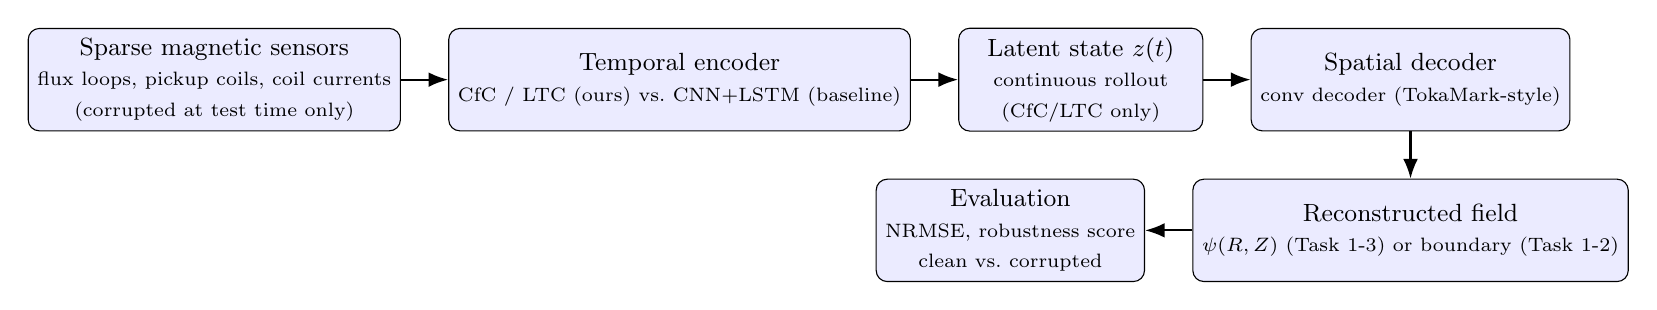
\begin{tikzpicture}[
      node distance=6mm and 6mm,
      box/.style={draw, rounded corners, minimum height=1.3cm, minimum width=3.1cm, align=center, fill=blue!8, font=\small},
      arr/.style={-{Latex[length=2.5mm]}, thick}
    ]
    \node[box] (sensors) {Sparse magnetic sensors\\ \scriptsize flux loops, pickup coils, coil currents\\ \scriptsize (corrupted at test time only)};
    \node[box, right=of sensors] (encoder) {Temporal encoder\\ \scriptsize CfC / LTC (ours) vs.\ CNN+LSTM (baseline)};
    \node[box, right=of encoder] (latent) {Latent state $z(t)$\\ \scriptsize continuous rollout\\ \scriptsize (CfC/LTC only)};
    \node[box, right=of latent] (decoder) {Spatial decoder\\ \scriptsize conv decoder (TokaMark-style)};
    \node[box, below=of decoder, minimum width=3.1cm] (output) {Reconstructed field\\ \scriptsize $\psi(R,Z)$ (Task 1-3) or boundary (Task 1-2)};
    \node[box, left=of output] (metrics) {Evaluation\\ \scriptsize NRMSE, robustness score\\ \scriptsize clean vs.\ corrupted};

    \draw[arr] (sensors) -- (encoder);
    \draw[arr] (encoder) -- (latent);
    \draw[arr] (latent) -- (decoder);
    \draw[arr] (decoder) -- (output);
    \draw[arr] (output) -- (metrics);
  \end{tikzpicture}}
  \end{center}
  \vspace{4pt}
  \small
  \textbf{Key differentiator vs.\ prior art:} this is a controlled,
  like-for-like substitution -- same task, same data, same decoder -- so the
  CNN+LSTM-vs-CfC/LTC comparison isolates the effect of the temporal
  encoder, under both clean and corrupted conditions.
\end{frame}

\begin{frame}{Proposed Methodology -- Sensor Corruption Protocol \& Loss}
  \small
  \textbf{Corruption scenarios} (applied to the test set only, after
  training on clean data -- following Gupta's train-clean/corrupt-at-test
  design):
  \begin{itemize}
    \setlength\itemsep{2pt}
    \item \textbf{Random dropout}: randomly zero a fraction (e.g.\ 10\% /
      25\% / 50\%) of sensor readings across channels and timesteps
    \item \textbf{Single-channel failure}: one full sensor channel (e.g.\ a
      flux loop) removed for the entire input window
    \item \textbf{Temporal gap}: a contiguous block of timesteps blanked
      out (simulating an acquisition dropout)
  \end{itemize}

  \vspace{4pt}
  \textbf{Continuous-time formulation.} The latent state evolves as a
  function of elapsed time, not step count:
  \[
    \frac{dz(t)}{dt} = f_\theta\big(z(t), x(t)\big), \qquad
    z(t) = z(t_0) + \int_{t_0}^{t} f_\theta\big(z(\tau), x(\tau)\big)\, d\tau .
  \]
  CfC solves this in closed form (no numerical solver), so a missing or
  delayed reading changes the elapsed-time input rather than silently
  shifting the sequence index, as it would for an LSTM.

  \vspace{4pt}
  \textbf{Loss (reconstruction, matching TokaMark's own metric):}
  \[
    \mathcal{L}_{\text{recon}} = \text{NRMSE}\big(\hat{\psi}(R,Z),\, \psi(R,Z)\big)
  \]
\end{frame}

% ---------------------------------------------------------------------------
\section{Uniqueness}
\begin{frame}{Uniqueness / Novelty / Contribution}
  \begin{itemize}
    \item Extends Gupta's (2026) sensor-corruption benchmarking methodology
      -- established for a \textbf{forecasting} task -- to a
      \textbf{spatial reconstruction} task (Task 1-2/1-3), a setting this
      evaluation approach appears \textbf{comparatively less studied} in.
    \item Applies a continuous-time encoder (CfC, contrasted with LTC) to
      plasma state reconstruction -- continuous-time models are established
      elsewhere in tokamak research (transport dynamics, disruption
      prediction) but their use for spatial reconstruction is
      \textbf{limited work} by comparison.
    \item A \textbf{controlled, like-for-like architectural comparison}
      (same data, same decoder, only the temporal encoder changes) against
      an existing model class that has already shown promise on tokamak
      time series (Arnold et al.'s Continuous CNN result), evaluated here
      under a robustness lens that prior work did not apply.
    \item The contribution is framed as a \textbf{robustness evaluation and
      comparison}, not a claim of a new state-of-the-art architecture: the
      standard CNN+LSTM baseline may already be adequately robust, and that
      would be a valid, reportable outcome of this study.
  \end{itemize}
\end{frame}

% ---------------------------------------------------------------------------
\section{Dataset \& Setup}
\begin{frame}{Dataset \& Experimental Setup}
  \small
  \textbf{Data source.} TokaMark / FAIR-MAST -- real experimental shots from
  MAST. Publicly streamable, no credentials required
  (\texttt{s3.echo.stfc.ac.uk}); only the magnetics + currents + flux-map
  signals needed for Task 1-3 (9 of 39 total signal types) are streamed, not
  the full $\sim$2\,TB archive.

  \vspace{4pt}
  \textbf{Tasks.} Task 1-3 (flux map $\psi(R,Z)$, primary) and Task 1-2
  (plasma boundary, secondary/simpler check), both already defined with
  published baselines by TokaMark.

  \vspace{4pt}
  \textbf{Baselines (real, published numbers to reproduce and compare against).}
  \begin{itemize}
    \setlength\itemsep{1pt}
    \item CNN: 0.148 (Task 1-3, random split) / 0.502 (temporal split)
    \item CNN+LSTM: 0.159 (Task 1-3, random split) / 0.257 (temporal split)
  \end{itemize}

  \vspace{4pt}
  \textbf{Corruption protocol.} Random dropout (10/25/50\%), single-channel
  failure, temporal gap -- applied to the test split only, following
  Gupta's clean-train / corrupt-test design (Section: Methodology).

  \vspace{2pt}
  \textbf{Environment.} Python 3.10, PyTorch 2.3 on a single NVIDIA A100 GPU,
using \texttt{ncps}~1.0.1 for the CfC/LTC cells.
\end{frame}

% ---------------------------------------------------------------------------
\section{Implementation Status}
\begin{frame}{Implementation Status / Preliminary Results}
  
  \vspace{4pt}
  \begin{itemize}
    \item[$\boxtimes$] TokaMark data loader set up, magnetics+currents+flux streamed (done -- verified on real shots by EDA)
    \item[$\square$] CNN/CNN+LSTM baselines reproduced (in progress -- Kaggle run pending; targets CNN 0.148 / CNN+LSTM 0.159)
    \item[$\square$] CfC/LTC encoder implemented
    \item[$\square$] Corruption protocol implemented (dropout, channel failure, temporal gap)
    \item[$\square$] Preliminary clean-vs-corrupted comparison
  \end{itemize}
  \vspace{8pt}
  \begin{center}
    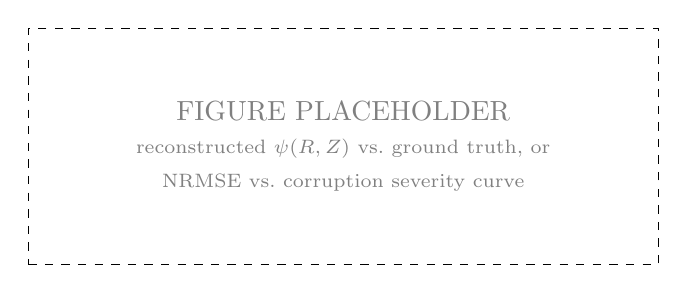
\begin{tikzpicture}
      \node[draw, dashed, minimum width=8cm, minimum height=3cm, align=center, text=gray]
        {FIGURE PLACEHOLDER\\ \scriptsize reconstructed $\psi(R,Z)$ vs.\ ground truth, or\\ \scriptsize NRMSE vs.\ corruption severity curve};
    \end{tikzpicture}
    % [FILL IN: path] -- \includegraphics[width=0.7\textwidth]{prelim_results.png}
  \end{center}
\end{frame}

% ---------------------------------------------------------------------------
\section{Challenges}
\begin{frame}{Challenges / Limitations}
  \begin{itemize}
    \item \textbf{Scope}: this project reconstructs one field (flux map or
      boundary), not the full multi-field plasma state (temperature,
      density, velocity together) -- a real limitation, left as future work.
    \item \textbf{Not full reactor control}: flux/boundary is one input a
      real control system needs, alongside temperature, density, and
      disruption precursors -- this project does not attempt control.
    \item \textbf{CfC implementation cost}: unlike LSTM, CfC is not a
      standard library layer; correct implementation needs care.
    \item \textbf{Baseline-number stability}: TokaMark's published numbers
      have already changed between paper revisions -- our reproduced
      baseline must be verified against the live version, not assumed.
    \item \textbf{Negative-result risk}: it is possible the discrete-time
      baseline is already adequately robust -- a valid, reportable outcome,
      not a failure of the project.
  \end{itemize}
\end{frame}

% ---------------------------------------------------------------------------
\section{Work Plan}
\begin{frame}{Work Plan \& Timeline}
  \scriptsize
  \renewcommand{\arraystretch}{1.15}
  \begin{tabular}{P{6.5cm}P{2.6cm}P{2.6cm}}
    \toprule
    \textbf{Task} & \textbf{Status} & \textbf{Owner(s)} \\
    \midrule
    Literature review \& gap finalization & Completed & Kalidasan \\
    TokaMark data pipeline setup (Task 1-2/1-3) & In progress & Nishanth \\
    Reproduce CNN / CNN+LSTM baselines & In progress & Kalidasan \\
    Implement CfC / LTC encoder & Remaining & Nishanth \\
    Implement corruption protocol & Remaining & Kalidasan \\
    E1: clean-data baseline reproduction & Remaining & Nishanth \\
    E2: robustness comparison under corruption & Remaining & Nishanth \\
    E3: temporal-split generalization check & Remaining & Kalidasan \\
    Result analysis \& writeup & Remaining & Nishanth \\
    Final report \& presentation & Remaining & Kalidasan \& Nishanth \\
    \bottomrule
  \end{tabular}
  \vspace{8pt}

  \footnotesize\textit{Baseline reproduction is expected to complete within the next 1--2 days,
  keeping the remaining experiments on track within the mid-review timeline.}
\end{frame}

% ---------------------------------------------------------------------------
\section{Expected Outcomes}
\begin{frame}{Expected Outcomes \& Evaluation Plan}
  \small
  \textbf{Metrics.} NRMSE (matching TokaMark's own metric, for direct
  comparability); a robustness score (relative degradation from clean to
  corrupted, following Gupta's framing).

  \vspace{4pt}
  \textbf{Experiments.}
  \begin{itemize}
    \item[E1] Reproduce CNN/CNN+LSTM baseline on clean data (correctness check)
    \item[E2] Corruption sweep (dropout / channel failure / temporal gap) -- CNN+LSTM vs.\ CfC/LTC
    \item[E3] Temporal-split evaluation (does continuous-time also help generalization, not just robustness)
  \end{itemize}

  \vspace{4pt}
  \begin{block}{Anticipated outcome (a comparison, not a predetermined result)}
    On clean data, CfC/LTC is anticipated to be comparable to CNN+LSTM (E1).
    Under corruption (E2), the explicit elapsed-time conditioning of
    continuous-time encoders \textbf{may} support more graceful degradation
    relative to the discrete-time baseline -- this is the hypothesis under
    test, not an assumed conclusion. Either outcome, including a negative
    result showing no meaningful difference, will be reported as a valid
    finding of this evaluation.
  \end{block}
\end{frame}

% ---------------------------------------------------------------------------
\section{References}
\begin{frame}[allowframebreaks]{References}
  \tiny
  \begin{itemize}
    \item Rousseau et al., ``TokaMark: A Comprehensive Benchmark for MAST Tokamak Plasma Models,'' arXiv:2602.10132, 2026.
    \item Boschi et al., ``TokaMind: A Multi-Modal Transformer Foundation Model for Tokamak Plasma Dynamics,'' arXiv:2602.15084, 2026.
    \item Gupta, ``Benchmarking Sensor Robustness in Plasma Diagnostic Models,'' arXiv:2607.11915, 2026.
    \item Arnold, Spangher \& Rea, ``Continuous Convolutional Neural Networks for Disruption Prediction in Nuclear Fusion Plasmas,'' arXiv:2312.01286, 2023.
    \item ``Fusion Equilibrium Challenge,'' arXiv:2609.01750 (NeurIPS-2026 benchmark), 2026.
    \item Yang et al., ``FusionMAE: pretrained model for fusion diagnostics,'' arXiv:2509.12945, 2025.
    \item Jalalvand et al., ``Multimodal Super-Resolution: Discovering Hidden Physics,'' \textit{Nat.\ Commun.}, 2025.
    \item ``Neural network reconstruction of the DIII-D tokamak plasma boundary using a reduced set of diagnostics,'' \textit{J.\ Plasma Phys.}, 2026.
    \item Joung et al., ``GS-DeepNet: mastering tokamak plasma equilibria with deep neural networks and the Grad-Shafranov equation,'' \textit{Sci.\ Rep.}, 2023.
    \item ``Application of Neural Ordinary Differential Equations for Tokamak Plasma Dynamics Analysis,'' arXiv:2403.01635, 2024.
    \item Rutigliano et al., ``Multi-diagnostics reconstruction of magnetic equilibrium and kinetic profiles using PINNs,'' \textit{Nucl.\ Fusion} 66:046006, 2026.
    \item Degrave et al., ``Magnetic control of tokamak plasmas through deep reinforcement learning,'' \textit{Nature}, 2022.
    \framebreak
    \item[] \textbf{Method background (cited in text):}
    \item Chen et al., ``Neural Ordinary Differential Equations,'' NeurIPS, 2018.
    \item Rubanova, Chen \& Duvenaud, ``Latent ODEs for Irregularly-Sampled Time Series,'' NeurIPS, 2019.
    \item Hasani et al., ``Liquid Time-constant Networks,'' AAAI, 2021.
    \item Hasani et al., ``Closed-form Continuous-time Neural Networks (CfC),'' \textit{Nat.\ Mach.\ Intell.}, 2022.
  \end{itemize}
\end{frame}

\end{document}
